\documentclass[10pt]{article}
\usepackage[utf8]{inputenc}
\usepackage{fixltx2e}
\usepackage{graphicx}
\usepackage{longtable}
\usepackage{booktabs}
\usepackage{amssymb}
\usepackage{mathpazo}
% \usepackage{fullpage}
% \usepackage{setspace}
\usepackage{amsmath, amssymb, amscd}
\usepackage{algorithm}
\usepackage{algorithmicx}
\usepackage{algpseudocode}
\def \minWordLength {31\ }
\def \corpusSize {6442}
\def \testSize {200}
\DeclareMathOperator*{\argmax}{arg\,max}
\title{Spam Classification of a Social Network}
\author{Jon-Michael Deldin \\ Artificial Intelligence Graduate Project}
\date{December 2012}
\usepackage{hyperref}
\hypersetup{
    bookmarks=true,         % show bookmarks bar?
    unicode=false,          % non-Latin characters in Acrobat’s bookmarks
    pdftoolbar=true,        % show Acrobat’s toolbar?
    pdfmenubar=true,        % show Acrobat’s menu?
    pdffitwindow=false,     % window fit to page when opened
    pdfstartview={FitH},    % fits the width of the page to the window
    pdftitle={Spam Classification of a Social Network},    % title
    pdfauthor={Jon-Michael Deldin},     % author
    pdfsubject={Artificial Intelligence},   % subject of the document
    pdfcreator={Jon-Michael Deldin},   % creator of the document
    pdfproducer={LaTeX}, % producer of the document
    pdfnewwindow=true,      % links in new window
    colorlinks=true,       % false: boxed links; true: colored links
    linkcolor=red,          % color of internal links (change box color with linkbordercolor)
    citecolor=green,        % color of links to bibliography
    filecolor=magenta,      % color of file links
    urlcolor=magenta           % color of external links
}
\begin{document}

\maketitle
\tableofcontents
% \doublespace
\section{Introduction}
Spam is a significant problem in online communities. Spammers advertise their
products, services, viruses, and more to members of these social networks.
Social networks are targeted because they are generally free, and the spammers
can advertise to users via direct messaging or indirect communication (e.g.,
comments on a post). This severely degrades the legitimate user's experience,
affects the website's search engine ranking, and tarnishes the website's
public image.

One social network suffering from spam is
AskNature\footnote{\url{http://www.asknature.org} }. AskNature is a free,
online database of biomimetic~\cite{benyus} solutions. Members can create a
profile, comment on articles, create and read articles, and participate in
forums. Unfortunately, spammers take advantage of the open user registration
and inundate the site with illegitimate accounts, such as the one shown in
Fig.~\ref{fig:spam-profile}. Since the site opened in November 2008, the staff
detected nearly 20,000 spam profiles, in contrast to almost 9,000 legitimate
profiles\footnote{As of November 28, 2012 }. The site has coped with a few
heuristics tools that check for links and HTML, but they are run only to
detect profiles -- a human still inspects and bans users.

\begin{figure}[t]
  \centering
  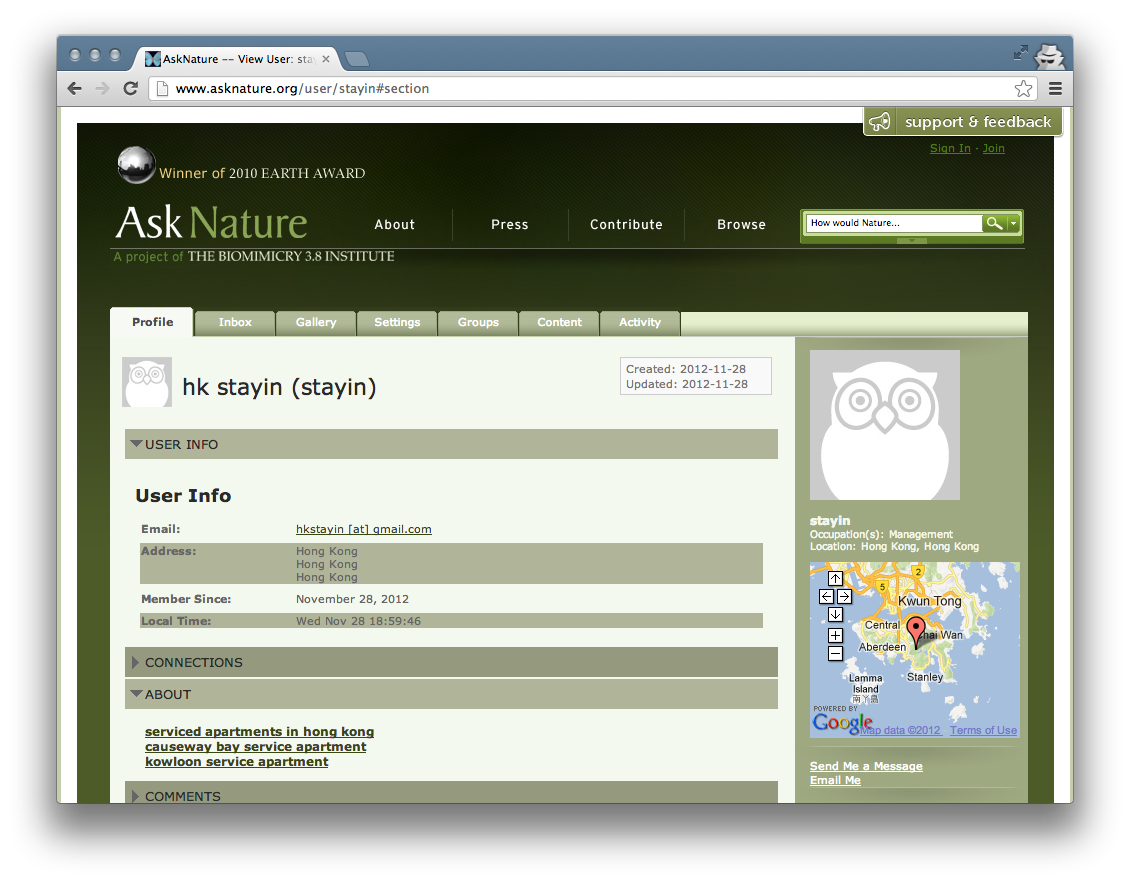
\includegraphics[width=\textwidth]{fig/spam-profile.png}
  \caption{This screenshot of a spam profile shows the "about" text the spammer
    enters, along with the first name ("hk"), last name ("stayin"), username
    ("staying"), and the spammer's address.}
  \label{fig:spam-profile}
\end{figure}

In this project, I will develop a naive Bayes classifier for detecting spam
profiles based on the user's biography. The goal will be to determine whether an
account is spam or ham (i.e., a legitimate account) based on the plain text of
the profile's biography. I hypothesize a unigram bag of words model will outperform (see
\S\ref{sect:eval}) character gram and phonogram models. Character gram models
may suffer from too large of a search space, while phonograms (words
represented phonetically) will have too narrow of a search space, leading to
increased false positives and false negatives.

\section{Naive Bayes Classifier}
The research presented here utilizes a naive Bayes classifier to classify spam
and ham biographies. These classifiers are very effective for classifying
documents~\cite[p182]{mitchell}, and they are widely used in email spam
filters~\cite{which-nb}. This classifier uses the maximum a posteriori
estimate to predict which class a document belongs to. The ``naive''
assumption is that each attribute is independent of another, which simplifies
computing a predicted class $v$ to
\[ v = \argmax_{x\in X}\ \Pr(x)\prod_i{\Pr(a_i|x)}, \]
where $X$ is the set of possible classes (e.g., spam and ham), and $a_i$ is an
attribute (i.e., a term)~\cite[p177]{mitchell}. The probability of an attribute given a class is
often computed as a maximum likelihood estimate ({\sc mle}):
\[ \Pr(a_i|x) = \frac{{\textsc{count}_x}(a_i)}{N_x}, \] where
$\textsc{count}_x$ returns the number of occurrences of $a_i$ in the vector of
attributes $<a_1, a_2, \ldots, a_d>$ belonging to class $x$, and $N_x$ is the total number of attributes
for class $x$~\cite[p177]{mitchell}.

{\sc mle} is not without its faults. When the number of times an event occurs
is small, the probability will be zero, which will overfit the data.
Fortunately, additive smoothing (Laplace smoothing) combats this by adding a
smoothing parameter $\alpha$\footnote{\url{http://ai-class.com}, Unit 5, Topic 21}:
\[ \Pr(a_i|x) = \frac{{\textsc{count}}_x + \alpha}{N_x + \alpha d} \]

In text classification, a bag-of-words model is typically used to capture the
frequency of each term appearing in a document. The attributes/terms are words
or characters broken up into $n$-grams, where a unigram corresponds to a
single word (e.g., bag = \{``not'': 1, ``secret'': 1\}), a bigram corresponds to two
words (e.g., bag = \{``not-secret'': 1\}), etc.

\section{Evaluation}
\label{sect:eval}
$k$-fold cross-validation, described in Algorithm~\ref{algo:crossvalidation},
is used to compare performance between classifiers. Cross-validation will
return a confusion matrix -- a table of false positives (ham marked as spam),
false negatives (spam marked as ham), true positives (spam), and true
negatives (ham)\footnote{For brevity, $fp$ will denote a false positive, $tn$
  will denote a true negative, and so on.}. This matrix results in the metrics
summarized in Table~\ref{table:metrics}. In this paper, high accuracy is
important because it will classify more spam and ham, but it should not come
at the cost of low precision (i.e., more legitimate users marked as spammers).
Thus, it is unlikely for there to be a clear winner, as it's often a tradeoff
between accuracy, precision, and recall. In the event of a tie or unclear
winner, the model that is easiest to compute will win, as this classifier will
be deployed as a background process on a commodity server.

\begin{table}[b]
  \centering
  \caption{Summary of evaluation metrics~\cite{eval}. Fewer false positives
    are represented by a higher precision, and fewer false negatives are
    represented by a higher recall rate.}
  \label{table:metrics}
  \begin{tabular}{lcl}
    \toprule
    Metric & Formula & Describes \\ \midrule
  accuracy & $\frac{tp + tn}{tp + fp + fn + tn}$ & correctly predicted classes \\
  precision & $\frac{tp}{tp + fp}$ & correctly predicted positive classes\\
  recall & $\frac{tp}{tp + fn}$ & how sensitive the classifier is to input \\\bottomrule
  \end{tabular}
\end{table}

\begin{algorithm}[t]
  \caption{$k$-fold cross-validation described by~\cite[p147]{mitchell}}
  \begin{algorithmic}
    \Function{CrossValidate}{data, $k$}
    \State partitions $\gets$ divide data into $k$ disjoint subsets
    \For{$i \gets 1 \to k$}
    \State{$T \gets$ data $\setminus\ \mathrm{partitions}_i$}
    \State{{\sc train}($T$)}
    \State{{\sc classify}($\mathrm{partitions}_i$)}
    \State \Return{confusion matrix}
    \EndFor
    \EndFunction
  \end{algorithmic}\label{algo:crossvalidation}
\end{algorithm}

\section{Corpus}
The data consist of user biographies -- Unicode text fields -- spanning
2008-09-03--2012-11-28. These profiles\footnote{``Profile'' and ``biography''
  will be used interchangeably from this point forward.} are from AskNature's
MySQL database, and the spam ones were manually annotated by AskNature staff
during that period. Procuring the corpus involves the following steps:

\begin{enumerate}
\item Select non-empty biographies from all active and banned (spam) users
\item Sanitize each biography according to Algorithm~\ref{algo:preprocess}
\item Save each biography to disk as plain text for easier distribution
\item Determine the mean biography length
\item Segment the samples into training and testing sets according to
  Algorithm~\ref{algo:segment}
\end{enumerate}

\subsection{Mean Biography Length}
In order to maximize the performance of a classifier, appropriate documents
must be selected. Empty samples are obviously not useful in classifying
profiles, and samples with one or two words are unlikely to add reliable
information. One way to determine a minimum count is to take the mean word
counts across spam and ham samples. As shown in
Table~\ref{table:corpus-stats}, the data include more spam accounts than ham,
and those spam accounts have fewer words per biography on average. The wide
standard deviation for both classes is explained by two factors: Users are not
required to fill out the biography field, and even if they choose to, no
stated length requirements exist. These results indicate the floor of the
minimum mean should be used avoid rejecting too much data. Applying a minimum
length of \minWordLength words per biography reduces the eligible samples down
to 4,702 spam entries and 1,740 ham entries.

\begin{table}[t]
  \centering
  \caption{Summary statistics for the non-empty biographies processed
    according to Algorithm~\ref{algo:preprocess}.}
  \label{table:corpus-stats}
  \begin{tabular}{lccc}
    \toprule
    Class & $N$ & Mean Length (words) & $\sigma$\\ \midrule
    Spam  & 18,498 & 31.1 & 85.8 \\
    Ham   & 3,271  & 61.1 & 96.2 \\
    \bottomrule
  \end{tabular}
\end{table}

\begin{algorithm}[b]
  \begin{enumerate}
  \item Sanitize all HTML by retaining just the \texttt{innerHTML} (the
    content between start and closing tags). For example, \texttt{<a
      href="http://example.com">link</a>} becomes \texttt{link}.
  \item Remove all URLs
  \item Replace excess whitespace with single spaces
  \end{enumerate}
  \caption{Preprocessing routine for biographies}
  \label{algo:preprocess}
\end{algorithm}

\begin{algorithm}[t]
  \caption{Segmenting the data samples into training and test sets}
  \label{algo:segment}
  \begin{enumerate}
  \item Create a list of all profiles and randomize it
  \item Select all entries with biographies of \minWordLength or more words
  \item For each class (ham and spam), randomly select 100 entries for testing
    and write to a new \texttt{pruned/testing} directory.
  \item Write the remaining samples to \texttt{pruned/training}
  \end{enumerate}
\end{algorithm}


\section{Methods}

% This paper is concerned with developing a naive Bayes classifier that
% maximizes accuracy and precision to capture more spammers and to minimize
% false positives based on user biographies. Unfortunately, these two metrics
% are unlikely to be simulatneously high because so many words are common across
% classes.

Word\footnote{%
  A word is defined by any Unicode string containing one or more alphabetic
  characters. This can be encoded as a case-insensitive Perl Compatible
  Regular Expression ({\sc pcre}): \texttt{/[a-z']+/i}.}, character, and
phonogram models were evaluated with a naive Bayes classifier. For each gram
type, the effect of a smoothing parameter of 1 was evaluated. Each model is a
different way of tokenizing a string. All words were evaluated, including
``stopwords'' like ``the'', ``is'', and ``at'' in order to retain phrases. In
character-grams, a gram is a Unicode character, and grams of length 1-5 were
evaluated. As an example of a character gram, the trigrams for ``naive'' are
``nai'', ``aiv'', and ``ive''. In phonograms, the gram is the phonetic
representation of a word. Phonograms were determined by the double-metaphone
algorithm~\cite{double-metaphone}, which reduced words to 12 consonant sounds.

\section{Results}

The results of cross-validating and testing word, character, and phonetic
models are presented in Tables~\ref{table:word-cv}--\ref{table:phono-t}.

\subsection{Word Grams}

Table~\ref{table:word-cv} shows the 10-fold cross-validation results for
unigram, bigram, and trigram word models. Trigrams with no smoothing yield the
highest accuracy of 93.7\%, but the precision is low at 92.1\%. In some
classifiers, this would be acceptable, but this model would cause too many
legitimate users to be banned. The model with both a high accuracy (above
90\%) and high precision is the unigram model with $\alpha = 1$. This only
resulted in 21 ham profiles being marked as spam, which is much more
acceptable than 390+ false positives. While this model is not great at
detecting spam in the cross-validation, it actually outperforms the other
word-grams on the \testSize\ test samples. Table~\ref{table:word-t} shows the
unigram model with $\alpha=1$ achieving 94\% accuracy and 94.9\% precision.

\begin{table}[t]
  \centering
  \caption{10-fold cross-validation confusion matrix for word-gram models ($N = \corpusSize$)}
  \label{table:word-cv}
  \begin{tabular}{lclllcccc}
    \toprule
    tokenizer & $\alpha$ & accuracy & precision & recall & $tp$ & $tn$ & $fp$ & $fn$ \\ \midrule
    unigram & 0 & 0.926 & 0.919 & 0.986 & 4536 & 1241 & 399 & 66 \\
    unigram & 1 & 0.905 & 0.995 & 0.876 & 4032 & 1619 & 21 & 570 \\
    bigram & 0 & 0.936 & 0.921 & 0.999 & 4599 & 1246 & 394 & 3 \\
    bigram & 1 & 0.563 & 0.996 & 0.409 & 1884 & 1632 & 8 & 2718 \\
    trigram & 0 & 0.937 & 0.921 & 0.999 & 4599 & 1247 & 393 & 3 \\
    trigram & 1 & 0.405 & 0.997 & 0.194 & 893 & 1637 & 3 & 3709 \\
    \bottomrule
  \end{tabular}
\end{table}

\begin{table}[b]
  \centering
  \caption{Word-gram confusion matrix for $N=\testSize$ test samples}
  \label{table:word-t}
  \begin{tabular}{lclllcccc}
    \toprule
    tokenizer & $\alpha$ & accuracy & precision & recall & $tp$ & $tn$ & $fp$ & $fn$ \\ \midrule
    unigram & 0 & 0.670 & 0.840 & 0.420 & 42 & 92 & 8 & 58 \\
    unigram & 1 & 0.940 & 0.949 & 0.930 & 93 & 95 & 5 & 7 \\
    bigram & 0 & 0.540 & 1 & 0.080 & 8 & 100 & 0 & 92 \\
    bigram & 1 & 0.700 & 1 & 0.400 & 40 & 100 & 0 & 60 \\
    trigram & 0 & 0.530 & 1 & 0.060 & 6 & 100 & 0 & 94 \\
    trigram & 1 & 0.600 & 1 & 0.200 & 20 & 100 & 0 & 80\\
    \bottomrule
  \end{tabular}
\end{table}

\subsection{Character Grams}

Table~\ref{table:char-cv} reports the 10-fold cross-validation matrix and
evaluation metrics for character grams of length 1-5\footnote{%
  Character grams longer than five characters were not pursued after
  disappointing results in an earlier experiment -- accuracy and precision
  decrease after four characters, and computing cross-validation matrices for
  larger grams takes a significant amount of computing power.}
  The best performing character-gram was a 4-gram with $\alpha = 1$
for a smoothing parameter. This model achieved 93.2\% accuracy and 99.2\%
precision in cross-validation, and 92.5\% accuracy and 95.7\% precision on the
test samples (Table~\ref{table:char-t}). The 5-gram with $\alpha=1$ model also
achieved the same results on the test samples, but given it's cross-validation
performance and the cost to compute, it is not the best character gram.

\begin{table}[b]
  \centering
  \caption{10-fold cross-validation confusion matrix for character-gram models ($N=\corpusSize$)}
  \label{table:char-cv}
  \begin{tabular}{lclllcccc}
    \toprule
    tokenizer & $\alpha$ & accuracy & precision & recall & $tp$ & $tn$ & $fp$ & $fn$ \\ \midrule
    1 & 0 & 0.696 & 0.882 & 0.679 & 3124 & 1221 & 419 & 1478 \\
    1 & 1 & 0.696 & 0.882 & 0.679 & 3125 & 1221 & 419 & 1477 \\
    2 & 0 & 0.855 & 0.948 & 0.851 & 3916 & 1424 & 216 & 686 \\
    2 & 1 & 0.862 & 0.969 & 0.840 & 3867 & 1516 & 124 & 735 \\
    3 & 0 & 0.881 & 0.901 & 0.943 & 4339 & 1162 & 478 & 263 \\
    3 & 1 & 0.926 & 0.986 & 0.912 & 4198 & 1580 & 60 & 404 \\
    4 & 0 & 0.911 & 0.900 & 0.990 & 4556 & 1131 & 509 & 46 \\
    4 & 1 & 0.932 & 0.992 & 0.915 & 4213 & 1605 & 35 & 389 \\
    5 & 0 & 0.931 & 0.915 & 0.999 & 4598 & 1215 & 425 & 4 \\
    5 & 1 & 0.897 & 0.865 & 3979 & 1619 & 21 & 623 \\
    \bottomrule
  \end{tabular}
\end{table}

% chars test

\begin{table}[b]
  \centering
  \caption{Character-gram confusion matrix for $N=\testSize$ test samples}
  \label{table:char-t}
  \begin{tabular}{lclllcccc}
    \toprule
    tokenizer & $\alpha$ & accuracy & precision & recall & $tp$ & $tn$ & $fp$ & $fn$ \\ \midrule
    1 & 0 & 0.710 & 0.728 & 0.670 & 67 & 75 & 25 & 33 \\
    1 & 1 & 0.710 & 0.728 & 0.670 & 67 & 75 & 25 & 33 \\
    2 & 0 & 0.830 & 0.837 & 0.820 & 82 & 84 & 16 & 18 \\
    2 & 1 & 0.865 & 0.884 & 0.840 & 84 & 89 & 11 & 16 \\
    3 & 0 & 0.800 & 0.806 & 0.790 & 79 & 81 & 19 & 21 \\
    3 & 1 & 0.915 & 0.919 & 0.910 & 91 & 92 & 8 & 9 \\
    4 & 0 & 0.645 & 0.738 & 0.450 & 45 & 84 & 16 & 55 \\
    4 & 1 & 0.925 & 0.957 & 0.890 & 89 & 96 & 4 & 11 \\
    5 & 0 & 0.580 & 0.900 & 0.180 & 18 & 98 & 2 & 82 \\
    5 & 1 & 0.925 & 0.957 & 0.890 & 89 & 96 & 4 & 11 \\
    \bottomrule
  \end{tabular}
\end{table}

\subsection{Phonograms}

Phonograms performed very poorly, as evidenced by Table~\ref{table:phono-cv}
and \ref{table:phono-t}. The best model was a single phonogram with no
smoothing, which achieved 79.5\% accuracy and 85.1\% precision in
cross-validation, but 61\% accuracy and precision in testing. The
two-phonogram model fared poorly with and without smoothing as well. It had
100\% recall, which came at the cost of 1,640 false positives.

% phono cv

\begin{table}[b]
  \centering
  \caption{10-fold cross-validation confusion matrix for phonograms ($N=\corpusSize$)}
  \label{table:phono-cv}
  \begin{tabular}{lclllcccc}
    \toprule
    tokenizer & $\alpha$ & accuracy & precision & recall & $tp$ & $tn$ & $fp$ & $fn$ \\ \midrule
    unigram & 0 & 0.795 & 0.851 & 0.875 & 4029 & 932 & 708 & 573 \\
    unigram & 1 & 0.558 & 0.737 & 0.623 & 2865 & 620 & 1020 & 1737 \\
    bigram & 0 & 0.737 & 0.737 & 1 & 4602 & 0 & 1640 & 0 \\
    bigram & 1 & 0.737 & 0.737 & 1 & 4602 & 0 & 1640 & 0 \\
    \bottomrule
  \end{tabular}
\end{table}
% phono test

\begin{table}[b]
  \centering
  \caption{Phonogram confusion matrix for $N=\testSize$ test samples}
  \label{table:phono-t}
  \begin{tabular}{lclllcccc}
    \toprule
    tokenizer & $\alpha$ & accuracy & precision & recall & $tp$ & $tn$ & $fp$ & $fn$ \\ \midrule
    unigram& 0 & 0.610 & 0.610 & 0.610 & 61 & 61 & 39 & 39 \\
    unigram& 1 & 0.610 & 0.610 & 0.610 & 61 & 61 & 39 & 39 \\
    bigram& 0 & 0.500 & 0.500 & 1 & 100 & 0 & 100 & 0 \\
    bigram & 1 & 0.500 & 0.500 & 1 & 100 & 0 & 100 & 0 \\

    \bottomrule
  \end{tabular}
\end{table}

\section{Discussion}

Of the best performing gram types, summarized in
Table~\ref{table:cv-sum}--\ref{table:t-sum}, both the 1-word gram and
4-character gram have high accuracy and precision. The word gram has higher
accuracy in testing with only one more false positive than the character gram.
However, according to the cross-validation results and the evaluation metrics
described in \S\ref{sect:eval}, the 1-word gram is superior due to it's ``good
enough'' accuracy and highest precision, and it is easy to compute. This
supports the hypothesis, but not clearly since character grams are very close.
Phonograms had low precision and recall, which also supports the hypothesis
that representing words phonetically will make the spam and ham vocabularies
too similar.

\begin{table}[b]
  \centering
  \caption{10-fold cross-validation comparison of the best performing gram
    models ($N=\corpusSize$)}
  \label{table:cv-sum}
  \begin{tabular}{lclllcccc}
    \toprule
    tokenizer & $\alpha$ & accuracy & precision & recall & $tp$ & $tn$ & $fp$ & $fn$ \\ \midrule
    1-word & 1 & 0.905 & 0.995 & 0.876 & 4032 & 1619 & 21 & 570 \\
    4-char & 1 & 0.932 & 0.992 & 0.915 & 4213 & 1605 & 35 & 389 \\
    1-phono& 0 & 0.795 & 0.851 & 0.875 & 4029 & 932 & 708 & 573 \\
  \end{tabular}
\end{table}

\begin{table}[h!]
  \centering
  \caption{Comparison of the best performing models on $N=\testSize$ test samples}
  \label{table:t-sum}
  \begin{tabular}{lclllcccc}
    \toprule
    tokenizer & $\alpha$ & accuracy & precision & recall & $tp$ & $tn$ & $fp$ & $fn$ \\ \midrule
    1-word gram & 1 & 0.940 & 0.949 & 0.930 & 93 & 95 & 5 & 7 \\
    4-char gram & 1 & 0.925 & 0.957 & 0.890 & 89 & 96 & 4 & 11 \\
    1-phono gram & 0 & 0.610 & 0.610 & 0.610 & 61 & 61 & 39 & 39 \\
  \end{tabular}
\end{table}

\section{Conclusion}

This paper developed a naive Bayes classifier for the AskNature social
network that classifies spam profiles with 94\% accuracy and 93\% precision
with a unigram word model. Both unigram word and 4-character gram models had
high accuracy and precision in 10-fold cross-validation of \corpusSize\
samples and testing on \testSize\ samples. Phonograms performed poorly as expected.

Future experiments may include combining the classifier developed here with
another classifier or heuristic to form an ensemble~\cite{ensemble}. A
weighted approach, where if one classifier returns a probability with some
uncertainty, the second classifier will run, and the maximum probability will
result in the prediction. This should reduce false positives and false
negatives. Another useful experiment would be on-line, continuous learning,
where the classifier is trained every time AskNature's staff tag a spam or ham
profile. Finally, varying the spam-to-ham ratio, as described in
Appendix~\ref{a:ratio} may be worth investigating to see what ratio of

\appendix
\section{Determining the Ratio of Spam to Ham}
\label{a:ratio}

Algorithm~\ref{algo:ratio} describes a method of evaluating all possible
spam-to-ham ratios from 1\% to 99\%, with the caveat that the best ratio is
influenced by a high accuracy and as high as possible precision. This
algorithm requires balanced training sets, which would substantially reduce
the number of spam entries. AskNature adds \textasciitilde 300 spam and
\textasciitilde 200 ham accounts each month, so this algorithm can be run once
there are more ham accounts with longer biographies.

\begin{algorithm}[h]
  \caption{Determine the ratio of spam:ham messages with the greatest accuracy.}
  \label{algo:ratio}
  \begin{algorithmic}
    \Function{FindBestRatio}{samples, $n$}
    \Comment{Takes a set of $n$ samples}
    \State spam $\gets$ {\sc shuffle}(samples $\setminus $ ham)
    \Comment{Randomizes the order of samples}
    \State ham $\gets$ {\sc shuffle}(samples $\setminus $ spam)
    \State best-accuracy $\gets 0$
    \State best-ratio $\gets \emptyset$
    \\

    \For{$i \gets 0.0 \to 1.0$, step $\gets 0.01$}
    \State ham-ratio $\gets ni$
    \State spam-ratio $\gets n(1 - i)$
    \State limited-samples $\gets$ {\sc take}(ham, ham-ratio) $\cup$ {\sc take}(spam, spam-ratio)
    \\

    \State {\sc cross-validate}(limited-samples)

    \If{accuracy $>$ best-accuracy}
    \State{best-accuracy $\gets$ accuracy}
    \State{best-ratio $\gets$ \{ham-ratio, spam-ratio\}}
    \EndIf
    \EndFor
    \State \Return{best-ratio, best-accuracy}
    \EndFunction
  \end{algorithmic}
\end{algorithm}

\section{Implementation}
\label{a:implementation}
The entire project is developed as a set of Ruby 1.9.3 and R scripts that are
glued together by a \texttt{Rakefile} for automation. The data files are
distributed as plain text files in the \texttt{src/data/processed} directory,
so a MySQL database is not needed to classify text. Since they need to be
accessed often, I have serialized them and saved them to disk for easy loading
in \texttt{src/data/objects}.

The following open-source libraries are used:

\begin{itemize}
\item Ankusa\footnote{\url{https://github.com/livingsocial/ankusa}}, an
  implementation of naive Bayes for text classification. I extended it in a
  number of ways. In terms of performance, I sped up word hashing and string
  conversion, resulting in 3-6 s improvement per classification, which adds up when
  cross-validating multiple models. For features, I implemented configurable
  Laplace smoothing and added n-gram support for word, character, and phonetic
  grams. I intend to contribute these changes upstream as soon as possible.
\item Text\footnote{\url{http://text.rubyforge.org}}, for the Double Metaphone
  implementation.
\item Parallel\footnote{\url{https://github.com/grosser/parallel}} for
  simplified multi-core and multi-threaded computing. My cross-validation
  routine is fully parallelized and uses six cores (configurable). My database
  import scripts are threaded, as they write thousands of files to disk.
  Wherever possible, I tried to parallelize my code because classifying text
  is really CPU intensive.
\item MySQL and Sequel\footnote{\url{http://sequel.rubyforge.org}} for
  accessing a database and fetching records.
\item Sanitize\footnote{\url{https://github.com/rgrove/sanitize}} for removing
  HTML.
\end{itemize}

Please consult
\texttt{src/README.md} for more details.

\bibliographystyle{plain}
\bibliography{refs}

\end{document}
